\RequirePackage{iftex}
\ifXeTeX\else
  \errmessage{This project must be compiled with XeLaTeX on Overleaf}
\fi
\documentclass[UTF8,a4paper,12pt,fontset=none]{ctexart}

\usepackage{geometry}
\usepackage{graphicx}
\usepackage{booktabs}
\usepackage{tabularx}
\usepackage{array}
\usepackage{amsmath}
\usepackage{float}
\usepackage{subcaption}
\usepackage{hyperref}
\usepackage{enumitem}
\usepackage{xcolor}
\usepackage{ifplatform}
\usepackage{fontspec}
\usepackage{xeCJK}

\ifwindows
  \setmainfont{Times New Roman}
  \setsansfont{Arial}
  \setmonofont{Consolas}
  \setCJKmainfont{SimSun}
  \setCJKsansfont{Microsoft YaHei}
  \setCJKmonofont{SimSun}
\else
  \setmainfont{TeX Gyre Termes}
  \setsansfont{TeX Gyre Heros}
  \setmonofont{TeX Gyre Cursor}
  \setCJKmainfont{Noto Serif CJK SC}
  \setCJKsansfont{Noto Sans CJK SC}
  \setCJKmonofont{Noto Sans CJK SC}
\fi

\geometry{left=2.4cm,right=2.4cm,top=2.6cm,bottom=2.6cm}
\setlength{\parskip}{0.45em}
\setlength{\parindent}{2em}
\setlist[itemize]{leftmargin=2.2em}
\hypersetup{
  colorlinks=true,
  linkcolor=black,
  citecolor=blue!60!black,
  urlcolor=blue!60!black
}

\title{InkPi：基于公开标准重构的楷书与行书单字书法辅助评测系统}
\author{Zongrui}
\date{2026年4月}

\begin{document}

\maketitle

\begin{abstract}
针对书法练习中“反馈周期长、评价口径不透明、设备端与云端脱节”的问题，本文设计并实现了一套面向毛笔楷书与行书单字练习的书法辅助评测系统 InkPi。系统以树莓派为设备端核心，采用 PyQt6 构建 3.5 寸小屏正式界面，在保持统一图像预处理与 OCR 入口不变的前提下，通过显式书体字段 \texttt{script} 将评测范围收敛为楷书与行书两种正式支持书体，并在 OCR 后按书体路由到对应 ONNX 主评分模型。与早期仅依赖“四维解释层”的做法不同，本文进一步基于教育部书法教育文件、地方书法水平测试大纲、中国美术学院社会美术水平考级标准以及中国书法家协会展览评审语境，重构了两套来源明确的五维正式评审标准：楷书标准强调笔法点画、结体字法、布白章法、墨法笔力与规范完整，行书标准强调用笔线质、结体取势、连带节奏、墨气笔力与规范识别。当前系统保持 \texttt{total\_score} 作为正式主分，同时将新的 rubric 直接用于结果展示、移动端查看、统计分析与方法论接口，并将 \texttt{rubric\_preview\_total} 仅保留为内部验证量。围绕该评测链路，InkPi 进一步实现了 Cloud API、运维后台、小程序和本地/云端数据库协同，使系统能够完成本地评测、结果同步、状态监控、移动端复盘和人工复评数据沉淀。本文重点介绍该系统的来源化评审标准、双书体运行架构、过渡期主分策略以及当前验证路线。
\end{abstract}

\noindent\textbf{关键词：} 书法评测；树莓派；OCR；ONNX；来源化评审标准；边缘云协同

\section*{Abstract}
InkPi is a Raspberry-Pi-centered calligraphy assistance system for single-character practice in regular script and running script. The system keeps image preprocessing and OCR shared across the whole runtime, while explicitly introducing a user-selected \texttt{script} field to route each sample to the corresponding ONNX scorer after OCR. In this iteration, the public-facing evaluation layer is rebuilt from an ad-hoc four-dimension explanation scheme into two source-backed five-dimension rubrics, one for regular script and one for running script. The new rubrics are grounded in publicly available education guidelines, local calligraphy test outlines, social art examination standards, and exhibition review discourse. InkPi keeps the current ONNX-based \texttt{total\_score} as the official primary score during the transition, while exposing the new rubric items in the device UI, cloud APIs, miniapp, and operations console. Around this evaluation pipeline, the project further integrates a PyQt6 device-side interface for a 3.5-inch screen, a Flask-based Cloud API, a monitoring-oriented web operations console, and a miniapp for history browsing, statistics, evidence inspection, and coaching-oriented feedback. This paper presents the source-backed rubric design, the dual-script runtime architecture, the transition strategy that keeps the legacy primary score unchanged for now, and the current validation path for future rubric-aware retraining.

\noindent\textbf{Keywords:} calligraphy assessment; Raspberry Pi; OCR; ONNX; source-backed rubric; edge-cloud system

\section{引言}
书法学习天然依赖教师示范与点评，但在初学者练习、课堂展示和设备端即时反馈场景中，这种模式常面临两个现实问题。其一，反馈周期较长，学生难以在一次练习后迅速获得稳定、结构化的改进建议；其二，评价口径往往停留在经验描述，例如“写得稳不稳”“结构好不好”，难以形成可追踪、可统计、可复盘的数字化结果。随着 OCR、边缘推理和多端同步能力的成熟，书法辅助评测系统已经具备工程落地基础，但如果评价维度缺乏来源约束，系统很容易被质疑为“模型自己定义标准”，从而削弱项目的专业性和说服力。

InkPi 当前要解决的问题，不只是“能不能给分”，而是“能不能在边缘设备上稳定运行，并给出有依据、可解释、可追踪的结果”。此前系统已经形成了树莓派 Qt 正式端、Cloud API、运维后台和微信小程序协同的完整链路，但结果解释层主要采用了“结构 / 笔画 / 完整 / 稳定”四维框架。这个框架适合工程调试与早期教学反馈，却不足以应对“标准从何而来”的追问。为此，本轮重构把公开可查的教育、考级、协会、展赛来源引入系统，直接将其落实为两套独立的五维正式评审标准。

这次重构坚持三条边界。第一，产品范围仍限定在毛笔楷书与行书单字，不扩展到隶书、草书、篆书或多字作品。第二，OCR 和预处理链路保持不变，书体仍由用户手动选择，系统不引入自动书体识别。第三，现阶段新的正式标准先替换维度层，不替换当前主分：\texttt{total\_score} 仍由现有 ONNX 模型输出，新的 \texttt{rubric\_preview\_total} 只作为内部验证量，用于后续重训准备。这样做的目的，是在不打断当前可运行主链的前提下，把评价标准先建立起来。

\section{来源依据与标准骨架}
\subsection{来源目录}
InkPi 当前的新标准只使用公开可查、且能落到单字书法练习场景的来源。表~\ref{tab:sources} 给出了当前锁定的来源目录。

\begin{table}[H]
  \centering
  \caption{InkPi 来源化标准目录}
  \label{tab:sources}
  \begin{tabularx}{\textwidth}{>{\raggedright\arraybackslash}p{2.1cm} >{\raggedright\arraybackslash}p{4.7cm} >{\raggedright\arraybackslash}p{3.1cm} X}
    \toprule
    来源码 & 来源名称 & 机构 & 在系统中的作用 \\
    \midrule
    MOE-2013 & 《中小学书法教育指导纲要》 \cite{moe2013} & 教育部 & 确立规范书写、技能训练、评价多元的教育边界。 \\
    MOE-2025 & 对十四届全国人大二次会议第4162号建议的答复 \cite{moe2025} & 教育部 & 给出 2022 课标口径下楷书到规范、通行行楷/行书的 progression。 \\
    SC-SHFA-2018 & 四川省书法水平测试毛笔书法测试大纲 \cite{sc2018} & 四川省教育考试院 & 提供适合初学者场景的笔法、字法、章法、卷面权重骨架。 \\
    CAA-EXAM-2018 & 全国美术考级软笔书法考试与培训标准 \cite{caa2018} & 中国美术学院社会美术水平考级中心 & 补强提按顿挫、线条力度、结构准确度、章法完善等标准表述。 \\
    CWA-REVIEW-2024 & 全国第十三届书法篆刻展评审评议 \cite{cwa2024} & 中国书法家协会相关评审语境 & 提供笔法、结构、章法、墨法、笔力、规范识别等正式评审话语。 \\
    \bottomrule
  \end{tabularx}
\end{table}

这些来源的使用方式并不是“照搬考级规则给机器打分”，而是把它们转化为三类约束：一是定义系统的教育边界，避免把辅助评测系统包装成自动考级器；二是给出能映射到当前单字产品的维度与权重语言；三是为未来的人工复评、数据标注和重训提供统一标准。

\subsection{楷书正式标准}
楷书标准 \texttt{regular\_rubric\_v1} 的五个正式维度如表~\ref{tab:regular-rubric} 所示。

\begin{table}[H]
  \centering
  \caption{楷书正式标准 \texttt{regular\_rubric\_v1}}
  \label{tab:regular-rubric}
  \begin{tabularx}{\textwidth}{>{\raggedright\arraybackslash}p{2.7cm} >{\raggedright\arraybackslash}p{2.0cm} >{\centering\arraybackslash}p{1.0cm} X}
    \toprule
    key & 展示名称 & 权重 & 主要依据 \\
    \midrule
    \texttt{bifa\_dianhua} & 笔法点画 & 30 & 四川“笔法”；国美“提按顿挫及线条力度”；中书协“笔法/笔力”。 \\
    \texttt{jieti\_zifa} & 结体字法 & 30 & 四川“字法”；国美“结构准确度”；教育部“规范书写/间架结构”。 \\
    \texttt{bubai\_zhangfa} & 布白章法 & 15 & 四川“章法”；中书协“章法/主次/不过度形式化”。 \\
    \texttt{mofa\_bili} & 墨法笔力 & 15 & 中书协“墨法、笔力”；国美“点画有力”。 \\
    \texttt{guifan\_wanzheng} & 规范完整 & 10 & 教育部“规范书写”；中书协“文字正误/写法不规范”；四川“卷面整洁”。 \\
    \bottomrule
  \end{tabularx}
\end{table}

需要说明的是，协会和展赛语境中的“章法”通常对应整幅作品布局，而 InkPi 当前只做单字练习。因此系统把这项适配为字内布白、重心位置、四边留白和字内疏密关系，而不把整幅作品章法强行压缩到单字界面中。

\subsection{行书正式标准}
行书标准 \texttt{running\_rubric\_v1} 的五个正式维度如表~\ref{tab:running-rubric} 所示。

\begin{table}[H]
  \centering
  \caption{行书正式标准 \texttt{running\_rubric\_v1}}
  \label{tab:running-rubric}
  \begin{tabularx}{\textwidth}{>{\raggedright\arraybackslash}p{2.7cm} >{\raggedright\arraybackslash}p{2.0cm} >{\centering\arraybackslash}p{1.0cm} X}
    \toprule
    key & 展示名称 & 权重 & 主要依据 \\
    \midrule
    \texttt{yongbi\_xianzhi} & 用笔线质 & 25 & 国美“提按顿挫、线条力度”；中书协“笔墨控制力”。 \\
    \texttt{jieti\_qushi} & 结体取势 & 20 & 教育部“规范、通行的行楷/行书”；中书协“结体与气息”。 \\
    \texttt{liandai\_jiezou} & 连带节奏 & 25 & 行书书体特征；中书协关于行草“气韵贯通”的评审语言。 \\
    \texttt{moqi\_bili} & 墨气笔力 & 20 & 中书协“墨法、笔力、气息”；国美“点画有力”。 \\
    \texttt{guifan\_shibie} & 规范识别 & 10 & 教育部规范书写边界；中书协“文字正误/写法不规范”。 \\
    \bottomrule
  \end{tabularx}
\end{table}

行书与楷书必须采用两套独立标准，而不能共享同一组维度名称和同一套解释文案。原因在于，楷书更强调结构、比例和起收笔稳定，行书则更强调连带、节奏和流动性下的可识别与可控性。InkPi 的重构核心之一，就是承认这种差异并将其做成运行时的一等逻辑。

\section{系统架构与双书体运行时}
InkPi 的整套架构如图~\ref{fig:system-flow} 所示。系统保留了统一的图像预处理和 OCR 入口，在 OCR 之后引入用户显式选择的 \texttt{script} 进行模型和评审标准路由。

\begin{figure}[H]
  \centering
  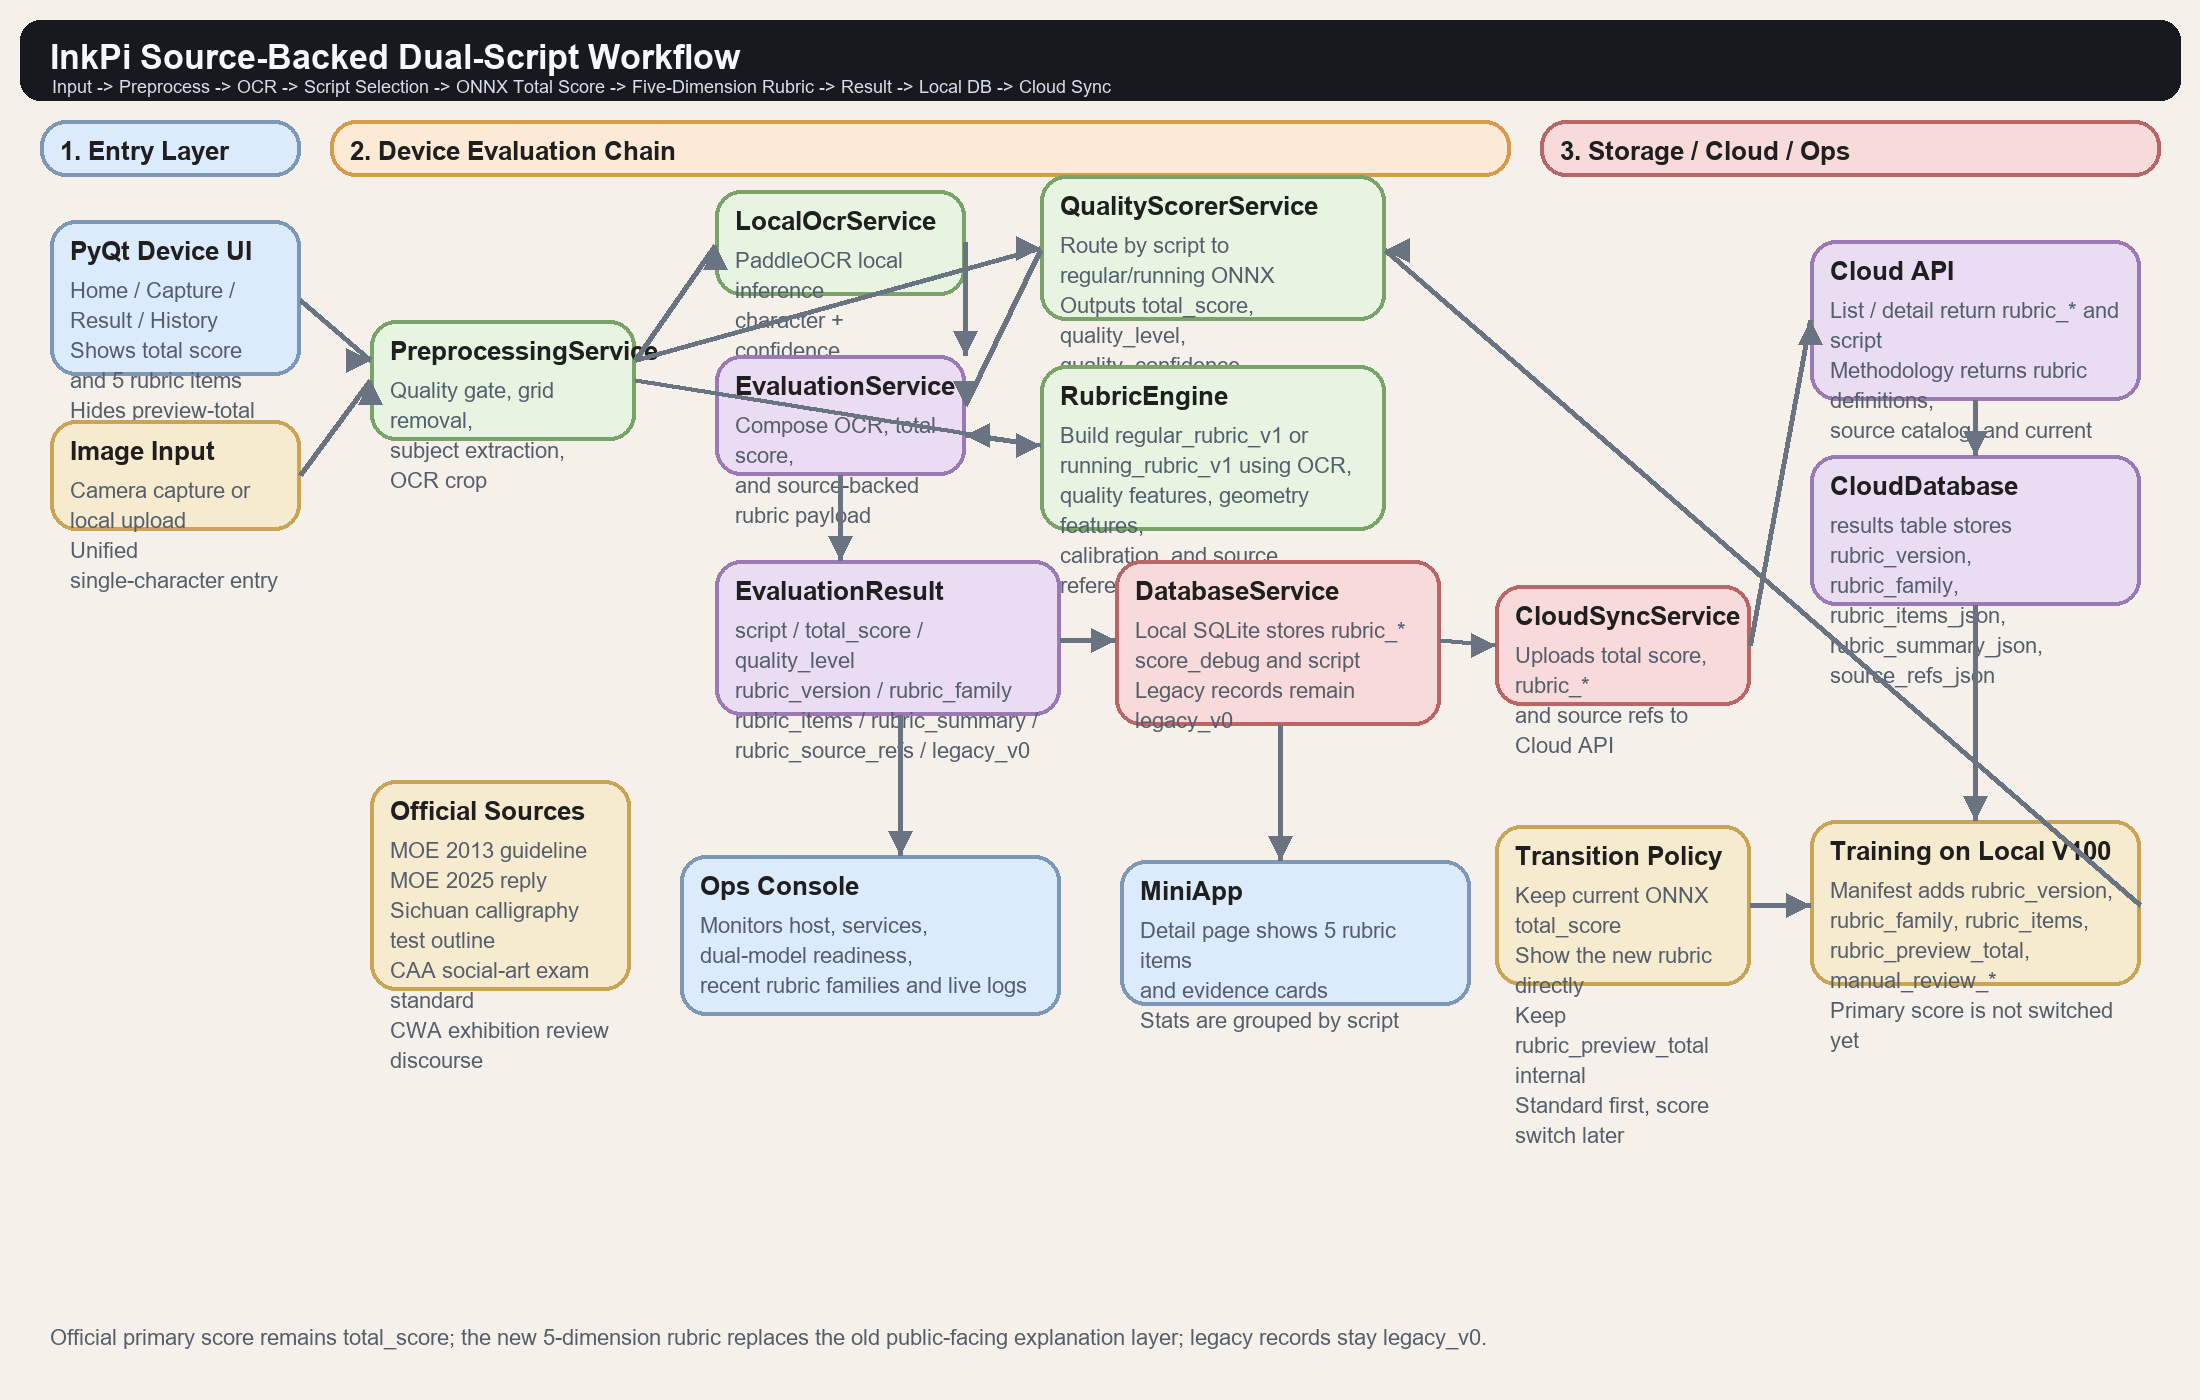
\includegraphics[width=\textwidth]{figures/system-flow.png}
  \caption{InkPi 当前主链与来源化 rubric 架构}
  \label{fig:system-flow}
\end{figure}

从职责划分看，系统由以下几层组成：

\begin{itemize}
  \item \textbf{Qt 设备端：} 面向 480x320 小屏，负责正式拍照、上传、书体选择、结果展示和历史浏览。
  \item \textbf{预处理与 OCR：} 统一执行预检、去网格、主体提取和单字识别，保持输入稳定。
  \item \textbf{双书体 ONNX 主分层：} 在 OCR 后按 \texttt{script} 路由到楷书或行书主分模型，继续输出当前 \texttt{total\_score}。
  \item \textbf{来源化 rubric engine：} 复用 OCR、几何特征、质量特征和校准中间量，生成五维正式评审项。
  \item \textbf{结果与存储层：} 统一装配为 \texttt{EvaluationResult}，写入本地 SQLite，再由云同步上传。
  \item \textbf{Cloud API 与小程序：} 负责历史、详情、方法论、验证总览、删除和人工复评。
  \item \textbf{运维后台：} 负责监控双模型 readiness、硬件状态、主机状态、日志和最近结果。
\end{itemize}

与很多“设备端和 Web 端都做同一套评测交互”的项目不同，InkPi 当前明确分离了正式端与运维端：Qt 只面向使用者和展示，Web 只面向状态观察与流程监控。这一设计让 3.5 寸小屏不被调试信息挤压，也让运维信息不会混入正式展示界面。

\section{来源化 rubric 与当前主分的关系}
\subsection{当前过渡策略}
本轮重构最关键的工程决策是：新标准直接上屏，但不立即切换正式主分。当前系统采用“两层评分”：

\begin{enumerate}
  \item 现有 ONNX 主分层继续输出 \texttt{total\_score}、\texttt{quality\_level} 和 \texttt{quality\_confidence}；
  \item 新的 rubric engine 生成五维正式评审项、依据说明和内部预览总分 \texttt{rubric\_preview\_total}。
\end{enumerate}

这样设计有两个好处。第一，设备侧、小程序、Cloud API 和运维后台可以立即切到来源化标准，解决“标准无源”的问题。第二，系统不会因为标准层重构同时引入主分漂移，从而影响已跑通的双书体主链。

\subsection{结果结构}
为支持这种过渡策略，\texttt{EvaluationResult} 当前新增了以下正式字段：

\begin{itemize}
  \item \texttt{rubric\_version}
  \item \texttt{rubric\_family}
  \item \texttt{rubric\_items}
  \item \texttt{rubric\_summary}
  \item \texttt{rubric\_source\_refs}
  \item \texttt{rubric\_preview\_total}
\end{itemize}

新记录写入 \texttt{rubric\_*}，旧记录则保留为 \texttt{legacy\_v0}。系统不会把旧的“四维结果”强行伪装成新的正式标准。这保证了历史兼容和标准切换的可追溯性。

\subsection{评分锚点}
当前 rubric engine 采用五档锚点机制：

\begin{equation}
s_i \in \{20, 40, 60, 80, 100\}
\end{equation}

每个维度分数都绑定来源化描述，而不是仅使用“优 / 良 / 中 / 差”的抽象标签。系统内部按照权重计算：

\begin{equation}
\texttt{rubric\_preview\_total} = \sum_i \left( \frac{w_i \cdot s_i}{100} \right)
\end{equation}

但在当前过渡阶段，这个内部总分不出现在 Qt、小程序和正式详情页中。对外仍然只有一个统一主分：\texttt{total\_score}。

\section{产品界面与多端协同}
\subsection{Qt 正式端}
图~\ref{fig:qt-ui} 给出了当前树莓派 Qt 正式界面的首页和结果页。新版 Qt 端面向 480x320 的 3.5 寸小屏做了收敛，只保留楷书与行书两个大书体入口，并直接显示新的五维正式评审项，而不是旧四维解释层。

\begin{figure}[H]
  \centering
  \begin{subfigure}[b]{0.46\textwidth}
    \centering
    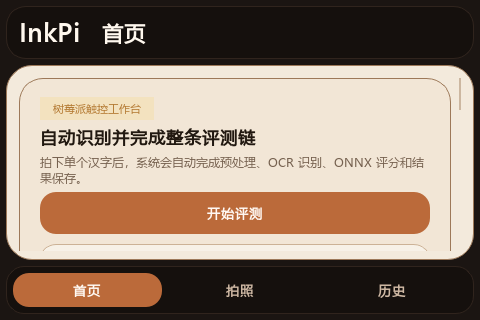
\includegraphics[width=\textwidth]{figures/qt-home.png}
    \caption{Qt 首页}
  \end{subfigure}
  \hfill
  \begin{subfigure}[b]{0.46\textwidth}
    \centering
    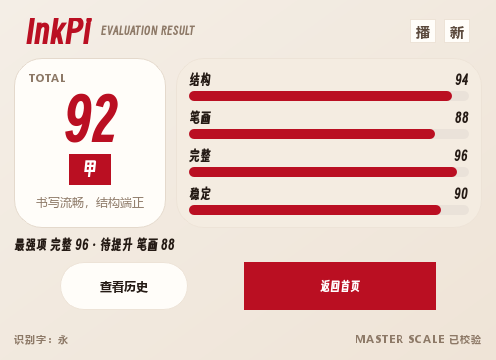
\includegraphics[width=\textwidth]{figures/qt-result.png}
    \caption{Qt 结果页}
  \end{subfigure}
  \caption{InkPi 树莓派正式界面}
  \label{fig:qt-ui}
\end{figure}

Qt 端当前展示的重点是：

\begin{itemize}
  \item 当前书体
  \item 统一主分 \texttt{total\_score}
  \item 五维正式评审项
  \item 依据化的简短建议
\end{itemize}

\subsection{Cloud API、小程序与运维后台}
Cloud API 不再只返回结果分数，还返回：

\begin{itemize}
  \item \texttt{rubric\_definitions}
  \item \texttt{rubric\_source\_catalog}
  \item \texttt{current\_script\_scope}
  \item \texttt{validation\_snapshot}
\end{itemize}

这使得小程序详情页和统计页可以直接展示新标准的来源、样本量、按书体维度均值和专家复评概览。与此同时，运维后台则重点呈现双模型 readiness、最近结果所属的 \texttt{rubric\_family}、流程事件和实时日志。换言之，这次标准重构并不是单纯改一个评分表，而是让来源化标准进入了整个产品链路。

\section{验证路线与训练准备}
\subsection{当前验证}
当前验证的重点不是证明“新的五维总分已经优于旧主分”，而是证明以下三点：

\begin{enumerate}
  \item 楷书与行书确实采用了两套独立标准；
  \item 新记录能完整写入 \texttt{rubric\_*}，旧记录能保留为 \texttt{legacy\_v0}；
  \item Qt、小程序、Cloud API 和运维后台都已切到新的五维正式标准层。
\end{enumerate}

当前项目已经具备以下量化出口：

\begin{itemize}
  \item 总样本量
  \item 覆盖汉字数
  \item 按书体的结果分布
  \item 设备来源
  \item 专家复评覆盖率
  \item AI 与人工一致率
  \item AI 与人工平均分差
\end{itemize}

这些指标已经进入 Cloud API 汇总接口和小程序统计页，因此项目后续答辩或汇报不再需要手工拼接验证数据。

\subsection{训练准备}
训练链路本轮只做准备性改造，不立即切换正式主分。manifest 中已经新增：

\begin{itemize}
  \item \texttt{rubric\_version}
  \item \texttt{rubric\_family}
  \item \texttt{rubric\_items}
  \item \texttt{rubric\_preview\_total}
  \item 人工评分对照字段
\end{itemize}

后续只有在以下条件同时满足时，才考虑用新标准重训并切换主分：

\begin{itemize}
  \item 楷书模型与行书模型都完成按新标准打标
  \item 人工对照验证通过
  \item 新旧主分切换的产品风险可控
\end{itemize}

\section{结论}
本文围绕 InkPi 项目给出了一套基于公开标准的双书体书法辅助评测系统方案。系统在保持 OCR 与预处理链路不变的前提下，把原先偏工程化的“四维解释层”重构为两套来源明确的五维正式评审标准，并将其统一接入树莓派 Qt 正式端、Cloud API、小程序和运维后台。与简单追求“能不能给出一个分数”相比，本轮重构更强调三件事：第一，标准必须有来源；第二，支持边界必须清楚；第三，标准层与主分层可以分阶段迁移，而不必一次性推翻当前已跑通的主链。

对 InkPi 而言，真正的价值不在于宣称“已经自动掌握书法评价”，而在于：它已经形成了一套可部署、可解释、可复核、可持续累积证据的辅助评测平台。后续工作将围绕新标准的人工对照、双书体重训、更多真实样本沉淀以及更完整的课堂应用展开。

\begin{thebibliography}{99}

\bibitem{moe2013}
中华人民共和国教育部.
\newblock 教育部关于印发《中小学书法教育指导纲要》的通知.
\newblock 2013.
\newblock Available: \url{https://hudong.moe.gov.cn/srcsite/A26/s8001/201301/t20130125_147389.html}.

\bibitem{moe2025}
中华人民共和国教育部.
\newblock 对十四届全国人大二次会议第4162号建议的答复.
\newblock 2025.
\newblock Available: \url{https://hudong.moe.gov.cn/jyb_xxgk/xxgk_jyta/jyta_jiaocaiju/202501/t20250113_1175495.html}.

\bibitem{sc2018}
四川省教育考试院.
\newblock 四川省书法水平测试毛笔书法测试大纲.
\newblock 2018.
\newblock Available: \url{https://www.sceeo.com/Html/201809/Newsdetail_817.html}.

\bibitem{caa2018}
中国美术学院社会美术水平考级中心.
\newblock 全国美术考级软笔书法考试与培训标准.
\newblock 2018.
\newblock Available: \url{https://mskj.caa.edu.cn/bkzn/kjdg/201809/33247.html}.

\bibitem{cwa2024}
中国文艺网.
\newblock 一步一个脚印——全国第十三届书法篆刻展览评审评议.
\newblock 2024.
\newblock Available: \url{https://www.cflac.org.cn/ys/sf/sfht/202405/t20240517_1316199.html}.

\bibitem{hui2007calligraphy}
Kaiyu Hui, Yue Gao, Yong Hu, and Songhua Xu.
\newblock An Intelligent System for Chinese Calligraphy.
\newblock In \emph{Proceedings of the Twenty-Second AAAI Conference on Artificial Intelligence}, 2007.
\newblock Available: \url{https://cdn.aaai.org/AAAI/2007/AAAI07-250.pdf}.

\bibitem{huda2020rpi}
Samsul Huda.
\newblock \emph{A Study of Raspberry Pi Applications to Calligraphy Learning and Air-Conditioning Guidance Systems}.
\newblock Okayama University, 2020.
\newblock Available: \url{https://ousar.lib.okayama-u.ac.jp/files/public/6/60936/20201203155610533257/K0006259_fulltext.pdf}.

\bibitem{yan2024siamese}
Fei Yan, Xueping Lan, Hua Zhang, and Linjing Li.
\newblock Intelligent Evaluation of Chinese Hard-Pen Calligraphy Using a Siamese Transformer Network.
\newblock \emph{Applied Sciences}, 14(5):2051, 2024.
\newblock Available: \url{https://www.mdpi.com/2076-3417/14/5/2051}.

\bibitem{xu2024penmanship}
Zebo Xu, Prerit S. Mittal, Mohd. Mohsin Ahmed, Chandranath Adak, and Zhenguang G. Cai.
\newblock Assessing penmanship of Chinese handwriting: a deep learning-based approach.
\newblock \emph{Reading and Writing}, 2024.
\newblock Available: \url{https://doi.org/10.1007/s11145-024-10531-w}.

\bibitem{paddleocr}
PaddlePaddle Authors.
\newblock PaddleOCR.
\newblock Available: \url{https://github.com/PaddlePaddle/PaddleOCR}. Accessed: 2026-04-19.

\bibitem{onnxruntime}
Microsoft.
\newblock ONNX Runtime.
\newblock Available: \url{https://onnxruntime.ai/}. Accessed: 2026-04-19.

\end{thebibliography}

\end{document}
